\documentclass{standalone}
\usepackage{tikz}
\usetikzlibrary{patterns, positioning}

\begin{document}
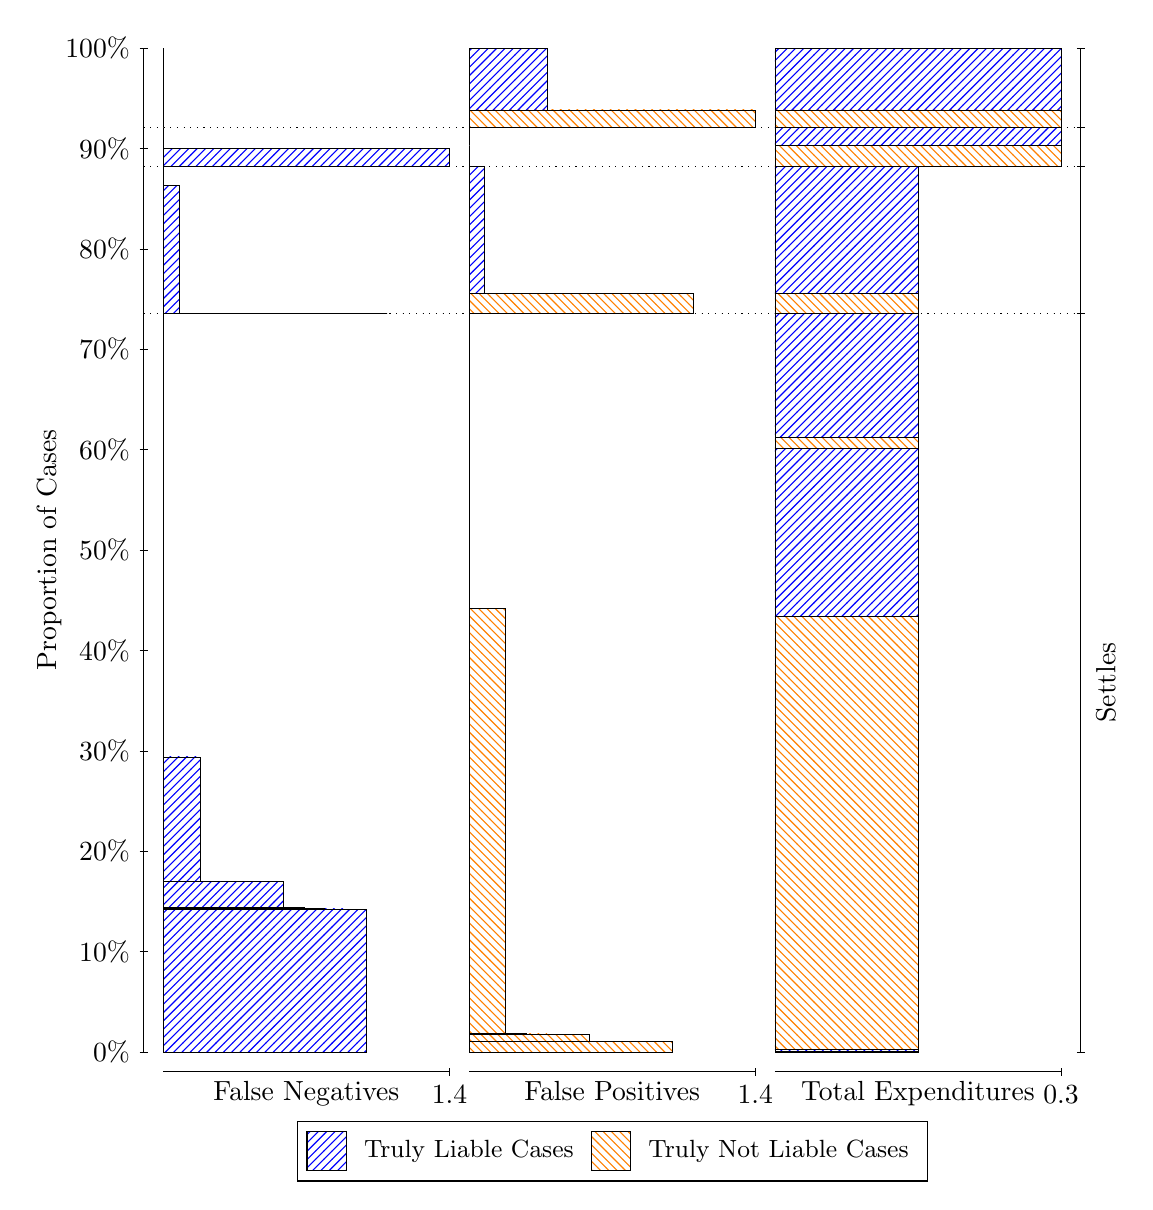
\begin{tikzpicture}
\draw[black, very thin] (1.5,1.75) -- (1.5,14.5);
\node[rotate=90, anchor=center] at (0.3, 8.125) {Proportion of Cases};
\draw[black, very thin] (1.45,1.75) -- (1.55,1.75);
\node[anchor=east] at (1.45, 1.75) {0\%};
\draw[black, very thin] (1.45,3.025) -- (1.55,3.025);
\node[anchor=east] at (1.45, 3.025) {10\%};
\draw[black, very thin] (1.45,4.3) -- (1.55,4.3);
\node[anchor=east] at (1.45, 4.3) {20\%};
\draw[black, very thin] (1.45,5.575) -- (1.55,5.575);
\node[anchor=east] at (1.45, 5.575) {30\%};
\draw[black, very thin] (1.45,6.85) -- (1.55,6.85);
\node[anchor=east] at (1.45, 6.85) {40\%};
\draw[black, very thin] (1.45,8.125) -- (1.55,8.125);
\node[anchor=east] at (1.45, 8.125) {50\%};
\draw[black, very thin] (1.45,9.4) -- (1.55,9.4);
\node[anchor=east] at (1.45, 9.4) {60\%};
\draw[black, very thin] (1.45,10.675) -- (1.55,10.675);
\node[anchor=east] at (1.45, 10.675) {70\%};
\draw[black, very thin] (1.45,11.95) -- (1.55,11.95);
\node[anchor=east] at (1.45, 11.95) {80\%};
\draw[black, very thin] (1.45,13.225) -- (1.55,13.225);
\node[anchor=east] at (1.45, 13.225) {90\%};
\draw[black, very thin] (1.45,14.5) -- (1.55,14.5);
\node[anchor=east] at (1.45, 14.5) {100\%};

\draw[black, very thin] (13.4,1.75) -- (13.4,14.5);
\draw[black, very thin] (13.35,1.75) -- (13.45,1.75);
\node[anchor=west] at (13.35, 1.75) {};
\draw[black, very thin] (13.35,11.133) -- (13.45,11.133);
\node[anchor=west] at (13.35, 11.133) {};
\draw[black, very thin] (13.35,11.133) -- (13.45,11.133);
\node[anchor=west] at (13.35, 11.133) {};
\draw[black, very thin] (13.35,12.999) -- (13.45,12.999);
\node[anchor=west] at (13.35, 12.999) {};
\draw[black, very thin] (13.35,13.488) -- (13.45,13.488);
\node[anchor=west] at (13.35, 13.488) {};
\draw[black, very thin] (13.35,14.5) -- (13.45,14.5);
\node[anchor=west] at (13.35, 14.5) {};

\draw[black, very thin, pattern color=blue, pattern=north east lines] (1.75,1.75) rectangle (4.3264,3.5589);
\draw[black, very thin, pattern color=blue, pattern=north east lines] (1.75,3.5589) rectangle (4.0621,3.5677);
\draw[black, very thin, pattern color=blue, pattern=north east lines] (1.75,3.5677) rectangle (3.7979,3.5772);
\draw[black, very thin, pattern color=blue, pattern=north east lines] (1.75,3.5772) rectangle (3.5336,3.5878);
\draw[black, very thin, pattern color=blue, pattern=north east lines] (1.75,3.5878) rectangle (3.2694,3.9191);
\draw[black, very thin, pattern color=blue, pattern=north east lines] (1.75,3.9191) rectangle (3.0052,3.9191);
\draw[black, very thin, pattern color=blue, pattern=north east lines] (1.75,3.9191) rectangle (2.7409,3.9191);
\draw[black, very thin, pattern color=blue, pattern=north east lines] (1.75,3.9191) rectangle (2.4767,3.9191);
\draw[black, very thin, pattern color=blue, pattern=north east lines] (1.75,3.9191) rectangle (2.2124,5.4971);
\draw[black, very thin, pattern color=orange, pattern=north west lines] (1.75,5.4971) rectangle (1.75,11.133);
\draw[black, very thin, pattern color=blue, pattern=north east lines] (1.75,11.133) rectangle (4.5906,11.133);
\draw[black, very thin, pattern color=orange, pattern=north west lines] (1.75,11.133) rectangle (1.75,11.133);
\draw[black, very thin, pattern color=blue, pattern=north east lines] (1.75,11.133) rectangle (1.9482,12.751);
\draw[black, very thin, pattern color=orange, pattern=north west lines] (1.75,12.751) rectangle (1.75,12.999);
\draw[black, very thin, pattern color=blue, pattern=north east lines] (1.75,12.999) rectangle (5.3833,13.224);
\draw[black, very thin, pattern color=orange, pattern=north west lines] (1.75,13.224) rectangle (1.75,13.488);
\draw[black, very thin, pattern color=orange, pattern=north west lines] (1.75,13.488) rectangle (1.75,13.715);
\draw[black, very thin, pattern color=blue, pattern=north east lines] (1.75,13.715) rectangle (1.75,14.5);
\draw[black, very thin, pattern color=orange, pattern=north west lines] (5.6333,1.75) rectangle (8.2097,1.8848);
\draw[black, very thin, pattern color=orange, pattern=north west lines] (5.6333,1.8848) rectangle (7.9455,1.8848);
\draw[black, very thin, pattern color=orange, pattern=north west lines] (5.6333,1.8848) rectangle (7.6812,1.8848);
\draw[black, very thin, pattern color=orange, pattern=north west lines] (5.6333,1.8848) rectangle (7.417,1.8848);
\draw[black, very thin, pattern color=orange, pattern=north west lines] (5.6333,1.8848) rectangle (7.1527,1.9745);
\draw[black, very thin, pattern color=orange, pattern=north west lines] (5.6333,1.9745) rectangle (6.8885,1.9745);
\draw[black, very thin, pattern color=orange, pattern=north west lines] (5.6333,1.9745) rectangle (6.8885,1.9773);
\draw[black, very thin, pattern color=orange, pattern=north west lines] (5.6333,1.9773) rectangle (6.6242,1.9799);
\draw[black, very thin, pattern color=orange, pattern=north west lines] (5.6333,1.9799) rectangle (6.36,1.9823);
\draw[black, very thin, pattern color=orange, pattern=north west lines] (5.6333,1.9823) rectangle (6.0958,7.3855);
\draw[black, very thin, pattern color=blue, pattern=north east lines] (5.6333,7.3855) rectangle (5.6333,11.133);
\draw[black, very thin, pattern color=orange, pattern=north west lines] (5.6333,11.133) rectangle (5.8315,11.133);
\draw[black, very thin, pattern color=blue, pattern=north east lines] (5.6333,11.133) rectangle (5.6333,11.133);
\draw[black, very thin, pattern color=orange, pattern=north west lines] (5.6333,11.133) rectangle (8.4739,11.381);
\draw[black, very thin, pattern color=blue, pattern=north east lines] (5.6333,11.381) rectangle (5.8315,12.999);
\draw[black, very thin, pattern color=orange, pattern=north west lines] (5.6333,12.999) rectangle (5.6333,13.263);
\draw[black, very thin, pattern color=blue, pattern=north east lines] (5.6333,13.263) rectangle (5.6333,13.488);
\draw[black, very thin, pattern color=orange, pattern=north west lines] (5.6333,13.488) rectangle (9.2667,13.715);
\draw[black, very thin, pattern color=blue, pattern=north east lines] (5.6333,13.715) rectangle (6.6242,14.5);
\draw[black, very thin, pattern color=orange, pattern=north west lines] (9.5167,1.75) rectangle (11.333,1.7578);
\draw[black, very thin, pattern color=blue, pattern=north east lines] (9.5167,1.7578) rectangle (11.333,1.7867);
\draw[black, very thin, pattern color=orange, pattern=north west lines] (9.5167,1.7867) rectangle (11.333,7.2795);
\draw[black, very thin, pattern color=blue, pattern=north east lines] (9.5167,7.2795) rectangle (11.333,9.4198);
\draw[black, very thin, pattern color=orange, pattern=north west lines] (9.5167,9.4198) rectangle (11.333,9.5546);
\draw[black, very thin, pattern color=blue, pattern=north east lines] (9.5167,9.5546) rectangle (11.333,11.133);
\draw[black, very thin, pattern color=orange, pattern=north west lines] (9.5167,11.133) rectangle (11.333,11.133);
\draw[black, very thin, pattern color=blue, pattern=north east lines] (9.5167,11.133) rectangle (11.333,11.133);
\draw[black, very thin, pattern color=orange, pattern=north west lines] (9.5167,11.133) rectangle (11.333,11.381);
\draw[black, very thin, pattern color=blue, pattern=north east lines] (9.5167,11.381) rectangle (11.333,12.999);
\draw[black, very thin, pattern color=orange, pattern=north west lines] (9.5167,12.999) rectangle (13.15,13.263);
\draw[black, very thin, pattern color=blue, pattern=north east lines] (9.5167,13.263) rectangle (13.15,13.488);
\draw[black, very thin, pattern color=orange, pattern=north west lines] (9.5167,13.488) rectangle (13.15,13.715);
\draw[black, very thin, pattern color=blue, pattern=north east lines] (9.5167,13.715) rectangle (13.15,14.5);
\draw[black, dotted] (1.5,11.133) -- (13.4,11.133);
\draw[black, dotted] (1.5,11.133) -- (13.4,11.133);
\draw[black, dotted] (1.5,12.999) -- (13.4,12.999);
\draw[black, dotted] (1.5,13.488) -- (13.4,13.488);
\draw[black, very thin] (1.75,1.5) -- (5.3833,1.5);
\node[anchor=north] at (3.5667, 1.5) {False Negatives};
\draw[black, very thin] (5.3833,1.45) -- (5.3833,1.55);
\node[anchor=north] at (5.3833, 1.45) {1.4};

\draw[black, very thin] (5.6333,1.5) -- (9.2667,1.5);
\node[anchor=north] at (7.45, 1.5) {False Positives};
\draw[black, very thin] (9.2667,1.45) -- (9.2667,1.55);
\node[anchor=north] at (9.2667, 1.45) {1.4};

\draw[black, very thin] (9.5167,1.5) -- (13.15,1.5);
\node[anchor=north] at (11.333, 1.5) {Total Expenditures};
\draw[black, very thin] (13.15,1.45) -- (13.15,1.55);
\node[anchor=north] at (13.15, 1.45) {0.3};

\node[black, centered, rotate=90] at (13.72, 6.4413) {Settles};





\draw (7.449999999999999,1.5) node[draw=none] (baseCoordinate) {};
\begin{scope}[align=center]
        \matrix[scale=0.5, draw=black, below=0.5cm of baseCoordinate, nodes={draw}, column sep=0.1cm]{
            \node[rectangle, draw, minimum width=0.5cm, minimum height=0.5cm, pattern=north east lines, pattern color=blue] {}; &
            \node[draw=none, font=\small] (B) {Truly Liable Cases}; &
            \node[rectangle, draw, minimum width=0.5cm, minimum height=0.5cm, pattern=north west lines, pattern color=orange] {}; &
            \node[draw=none, font=\small] (B) {Truly Not Liable Cases}; \\
            };
\end{scope}

\end{tikzpicture}
\end{document}